% ********** Rozdział 3 **********
\chapter{Przedstawienie realizacji projektu}
\section{Realizacja projektu}
Przedstawienie realizacji projektu "System Zarządzania Symulacją Samochodu" jest stworzony w programie Visual Studio 2022 w języku C\#. W tej części przedstawiam diagram Gantta.
\begin{figure}[!ht]
	\centering
		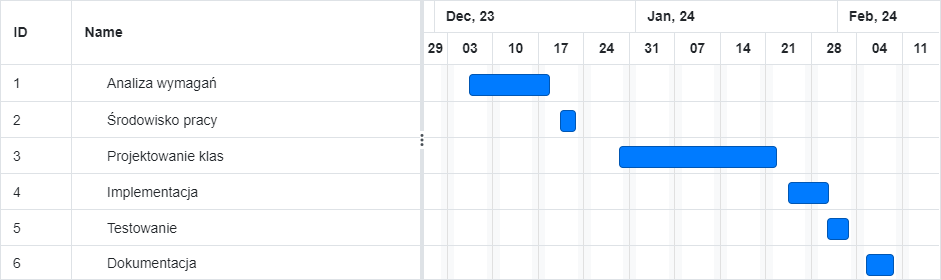
\includegraphics[width=17cm]{Diagram Gantta.png}
	\caption{\footnotesize Diagram Gantta}
	\label{fig:plotend}
\end{figure}

\begin{itemize}
\item Analiza wymagań: Proces polegający na ustaleniu konkretnych wymagań dla systemu zarządzania symulacją samochodu. Wymaga to dokładne zrozumienie i zebranie informacji potrzebnych do działania aplikacji.
\item Środowisko pracy: To miejsce, w którym przygotowuje się stanowisko programistyczne poprzez zainstalowanie odpowiednich pakietów środowiska i narzędzi na komputerze. Po przygotowaniu można przystąpić do tworzenia projektu.
\item Projektowanie klas: Etap projektowania obiektowego, podczas którego definiuje się klasy, ich właściwości i metody, aby zorganizować i strukturyzować kod źródłowy. W przypadku symulacji zachowania samochodu może to obejmować klasy reprezentujące różne aspekty samochodu.
\item Implenetacja: Proces przekształcania projektu i koncepcji klas w działający kod źródłowy, który realizuje określone funkcjonalności i spełnia wymagania użytkowników. W symulacji zachowania samochodu może to oznaczać implementację logiki sterującej zachowaniem samochodu.
\item Testowanie: Proces sprawdzania poprawności i skuteczności aplikacji poprzez wykonywanie testów na różnych etapach tworzenia. Testowanie symulacji zachowania samochodu może obejmować symulację różnych scenariuszy drogowych i sprawdzenie, czy samochód zachowuje się zgodnie z oczekiwaniami.
\item Dokumentacja: Tworzenie dokumentacji, która opisuje projekt, jego funkcjonalności, strukturę kodu źródłowego, sposób korzystania z aplikacji 
\end{itemize}

\section{Repozytorium i system kontroli wersji}
Projekt znajdujący się na stronie GitHub posiada wiele możliwości, które mogą być wykorzystane w celu monitorowania kodu.
Repozytorium znajduje się pod adresem:

\textbf {https://github.com/rafalwaz/System-zarzadzania-symulacja-samochodu}

\section{Prezentacja warstwy użytkowej projektu}
Zaprojektowanie warstwy użytkowej projektu "System Zarządzania Symulacją Samochodu" w sposób prosty, czytelny i łatwy dla użytkownika oraz wyeksponowanie funkcji działania rzeczywistej symulacji w interfejsie są kluczowe dla zapewnienia płynnej interakcji oraz maksymalnego zrozumienia procesu symulacji przez użytkowników. Ten podejście pozwoli użytkownikom szybko i efektywnie korzystać z systemu, co z kolei zwiększy ich satysfakcję i zaufanie do jego możliwości.

\begin{figure}[!ht]
	\centering
		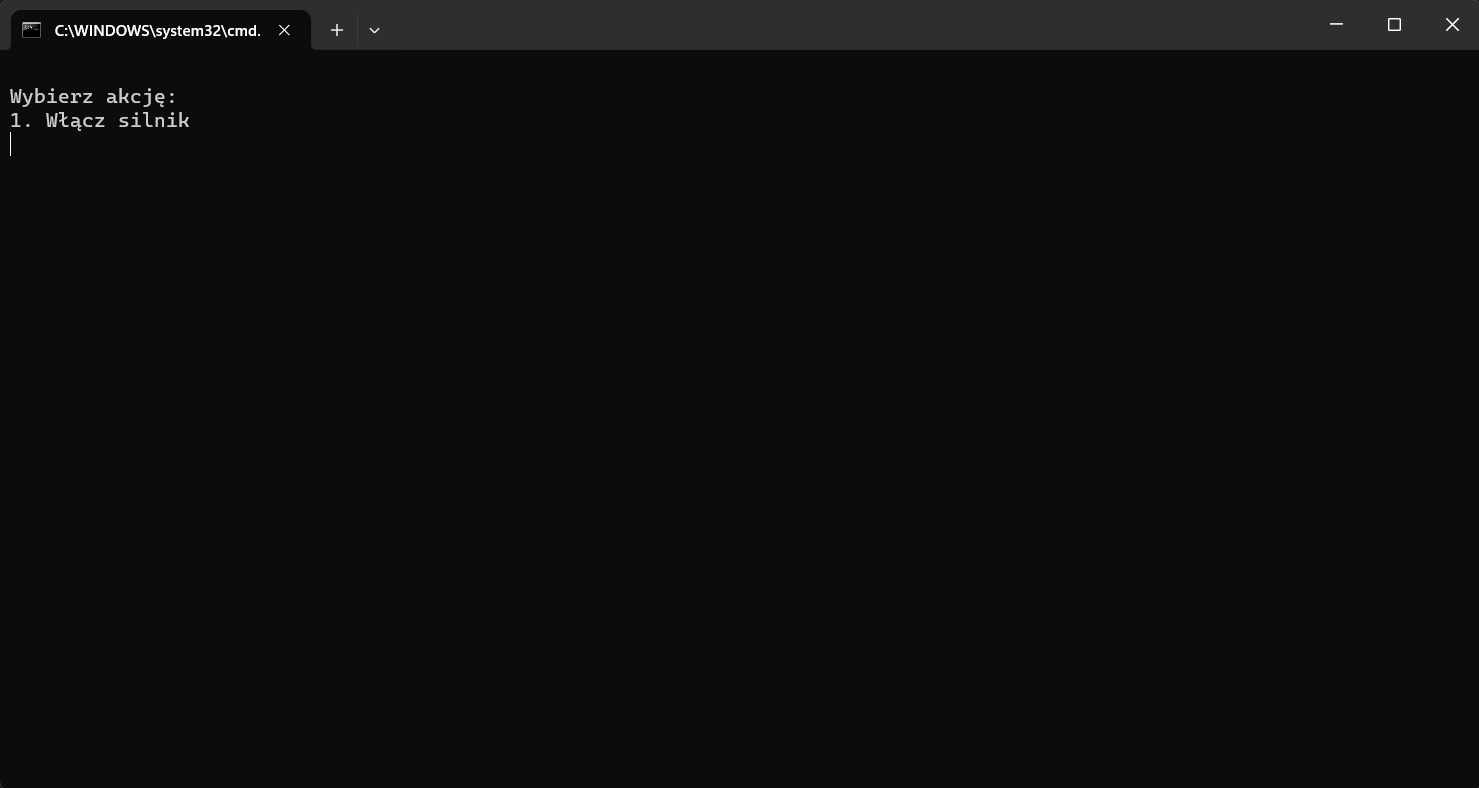
\includegraphics[width=17cm]{Włącz silnik.png}
	\caption{\footnotesize Włącz silnik}
	\label{fig:plotend}
\end{figure}

Uruchamiając program w konsoli wyświetla się informacja, która za pomocą przycisku numer 1 na klawiaturze wybierze akcje włącz silnik.
\newpage
Po wybraniu opcji na klawiaturze, użytkownik widzi w aplikacji włączony silnik, stan oleju, stan paliwa, pojemność w baku, aktulany stan silnika, aktualny bieg, prędkość, obroty silnika, ilość paliwa. 

\begin{figure}[!ht]
	\centering
		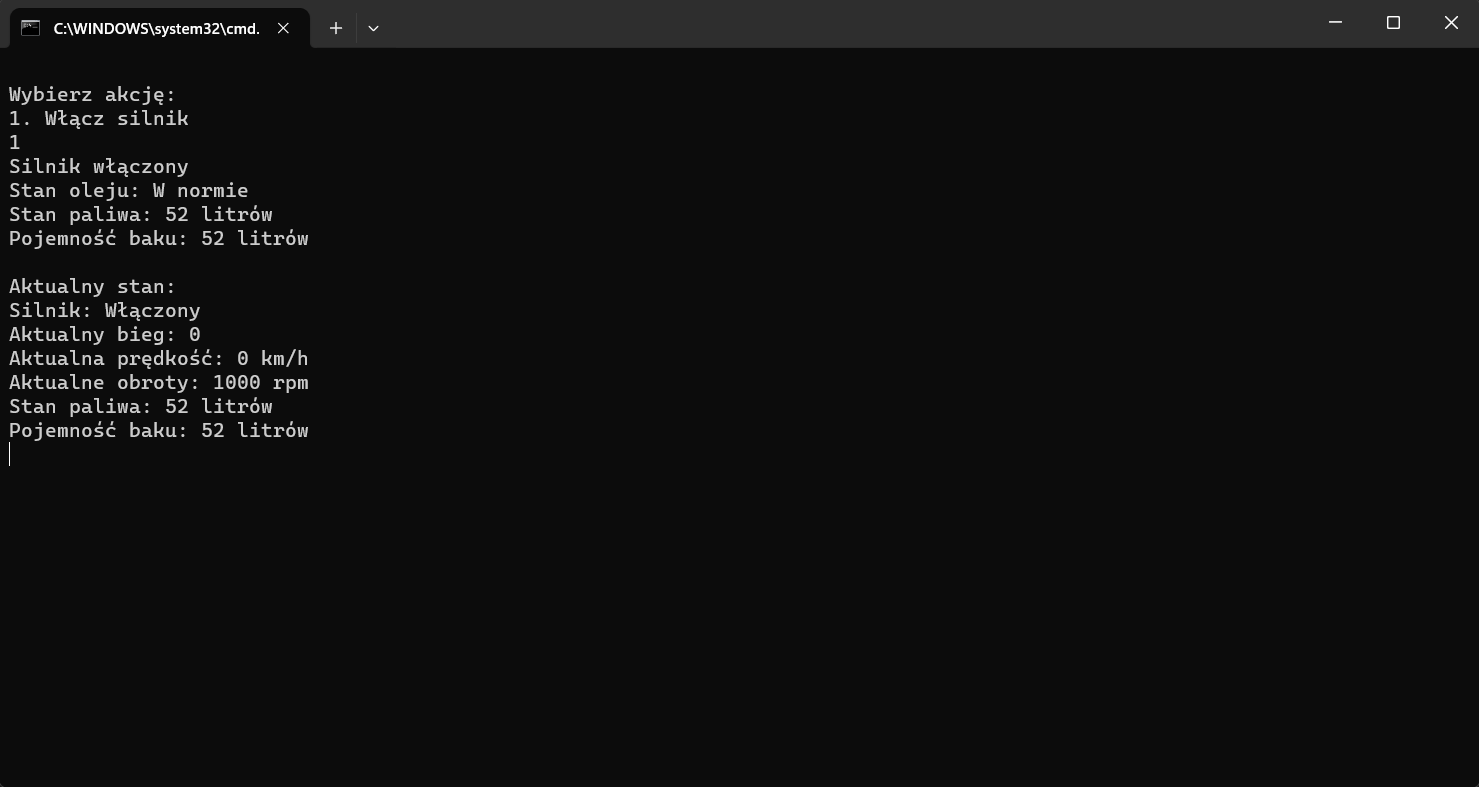
\includegraphics[width=17cm]{Włączony silnik.png}
	\caption{\footnotesize Włączony silnik}
	\label{fig:plotend}
\end{figure}
 
W sytuacji kiedy chcemy rozpocząć jazde na konsoli jest do wyboru opcja numer 2 która wskazuje przyśpieszenie samochodu 

\begin{figure}[!ht]
	\centering
		\includegraphics[width=17cm]{Wybór akcji.png}
	\caption{\footnotesize Wybór akcji}
	\label{fig:plotend}
\end{figure}

\newpage
Następnie w konsoli wystąpiła zmiana, kiedy przyśpieszono aktualna prędkość osiągneła 10km/h.  

\begin{figure}[!ht]
	\centering
		\includegraphics[width=17cm]{Przyśpieszenie.png}
	\caption{\footnotesize Przyśpieszenie}
	\label{fig:plotend}
\end{figure}
W konsoli wystąpiła zmiana aktualnie samochód porusza się na trzecim biegu. 
\begin{figure}[!ht]
	\centering
		\includegraphics[width=17cm]{Zmiana biegów.png}
	\caption{\footnotesize Zmiana biegów}
	\label{fig:plotend}
\end{figure}
\newpage
Aktualna prędkość 100km/h, zużycie paliwa 0,1 litrów. Na piątym biegu obroty silnika w tym momencie mają 3100 rpm. Stan paliwa na ten moment wynosi 41,9 litrów. Zużycie paliwa przy tej prędkości pokazuje 0,1 litrów, na takiej jeździe przewidywana ilość kilometrów na aktualnym stanie paliwa przewiduje 471km.
W przypadku kiedy trasa od Rzeszowa do Kielnarowej wynosi 17km przy prędkości 100km/h, średnia prędkość w przybliżeniu jest 86,84 km/h natomiast czas podróży będzie wynosił 11 minut 44 sekundy.

\begin{figure}[!ht]
	\centering
		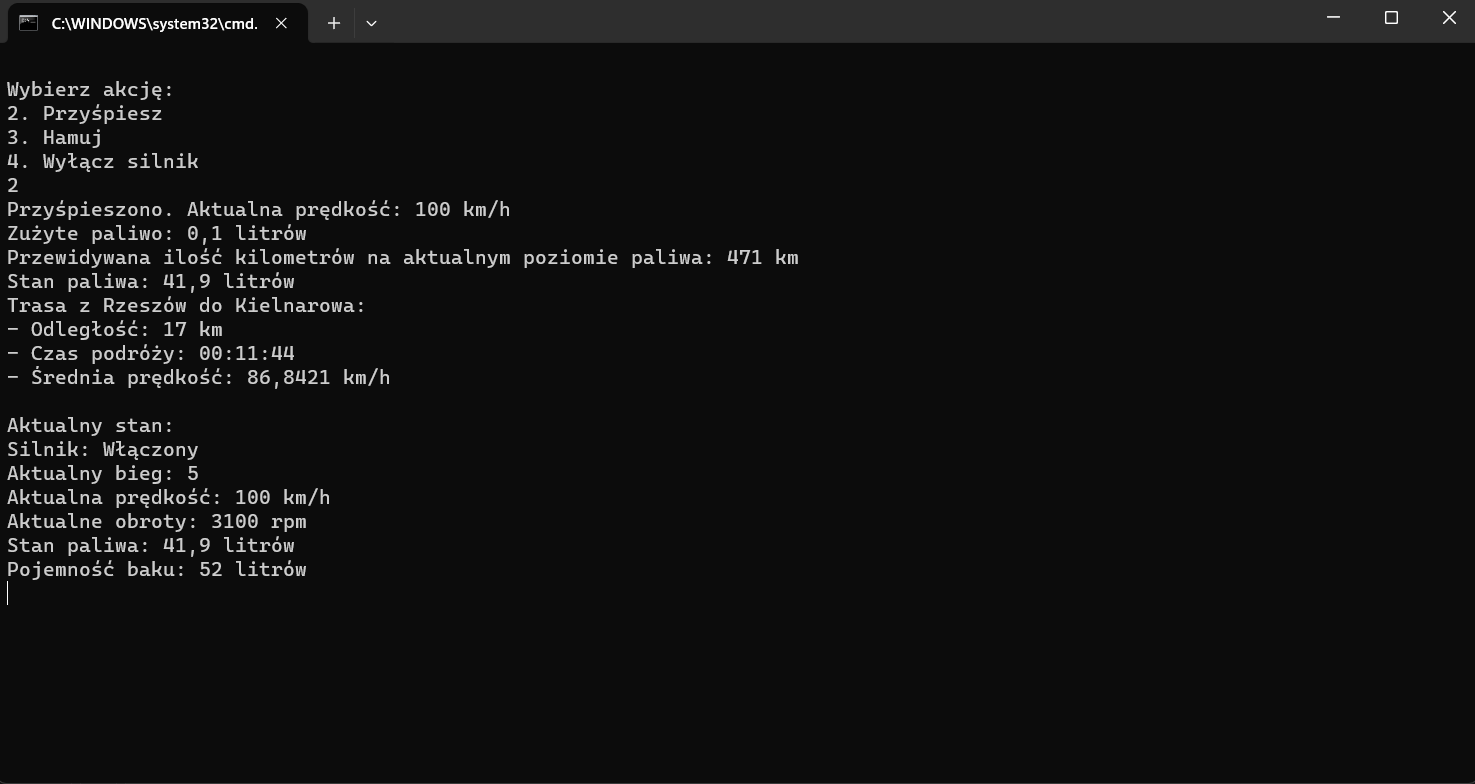
\includegraphics[width=17cm]{Parametry.png}
	\caption{\footnotesize Wyświetlenie parametrów}
	\label{fig:plotend}
\end{figure}

Jeżeli na konsoli użytkownik wybierze akcję numer 3, spowoduje hamowanie samochodu i automatycznie spadną obroty silnika i prędkość oraz bieg w tym przypadku zostanie zmieniony o jeden mniejszy. 

\begin{figure}[!ht]
	\centering
		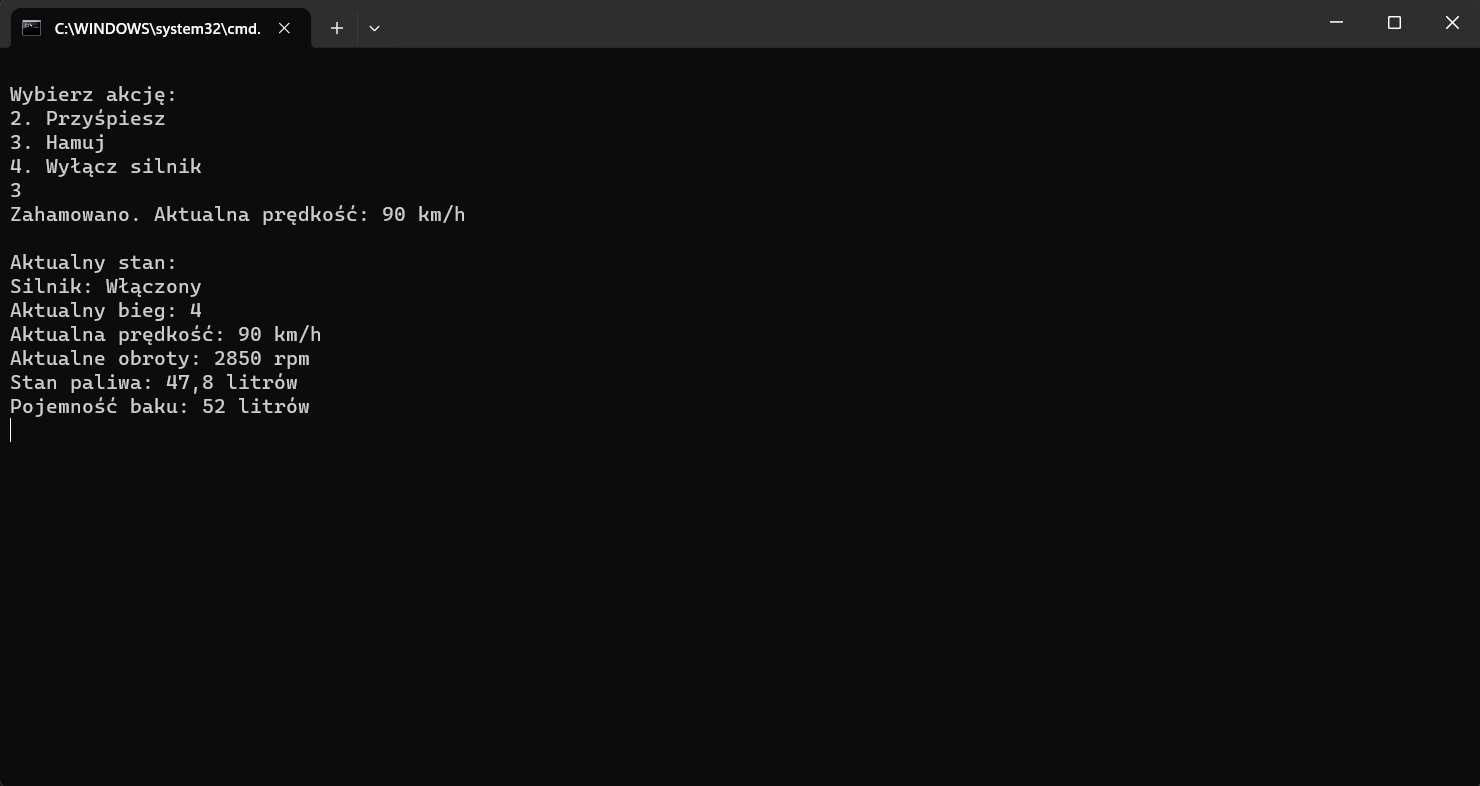
\includegraphics[width=17cm]{Hamowanie.png}
	\caption{\footnotesize Hamowanie}
	\label{fig:plotend}
\end{figure}
\newpage
W przypadku kiedy użytkownik zużyje paliwo a stan paliwa będzie wynosił 0 litrów. Wyświetli się informacja o braku paliwa i tym samym dalsza jazda nie będzie możliwa.

\begin{figure}[!ht]
	\centering
		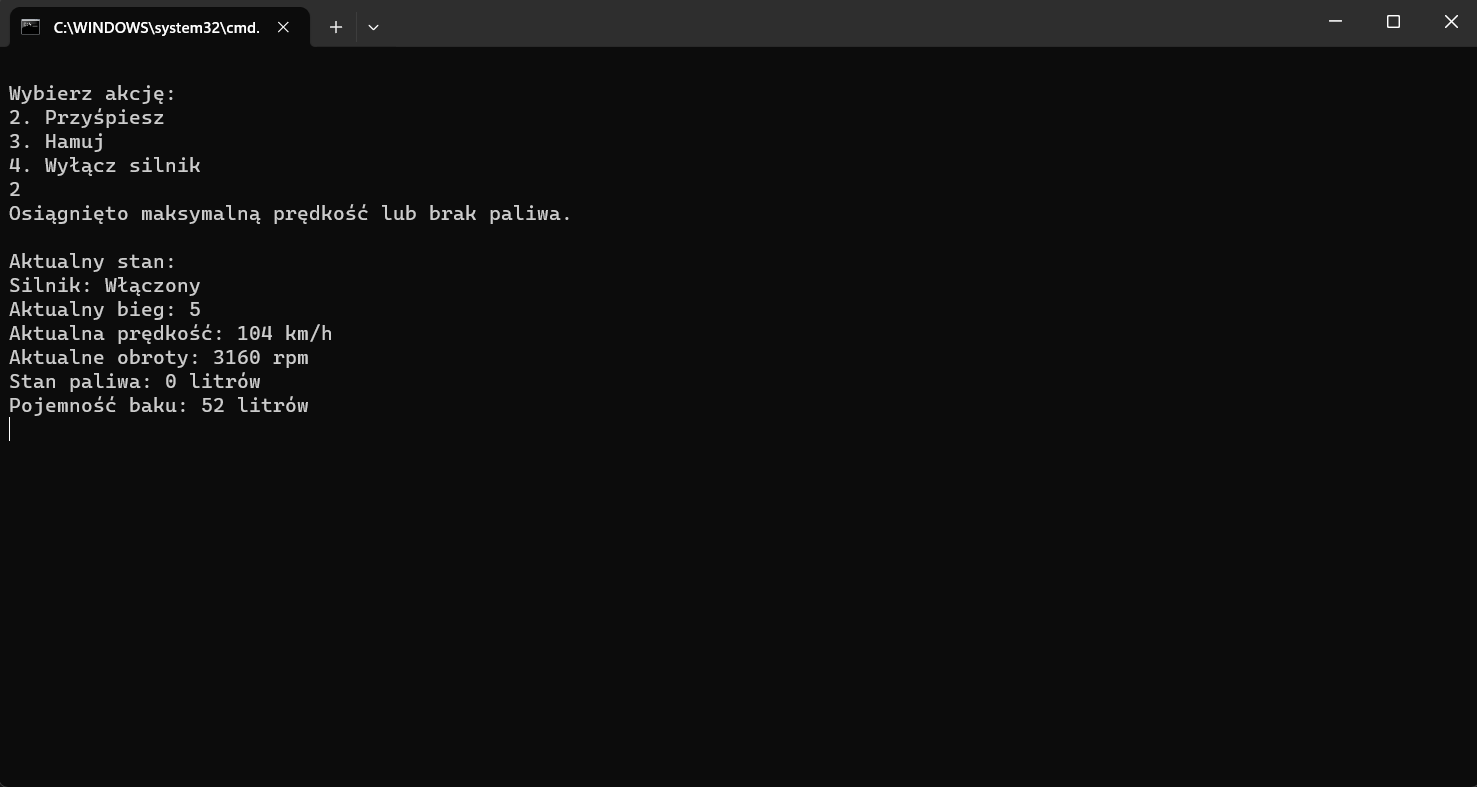
\includegraphics[width=17cm]{Brak paliwa.png}
	\caption{\footnotesize Brak paliwa}
	\label{fig:plotend}
\end{figure}

Kiedy użytkownik chce zakończyć jazde na consoli wybierze akcję numer 4 wyłącz silnik.

\begin{figure}[!ht]
	\centering
		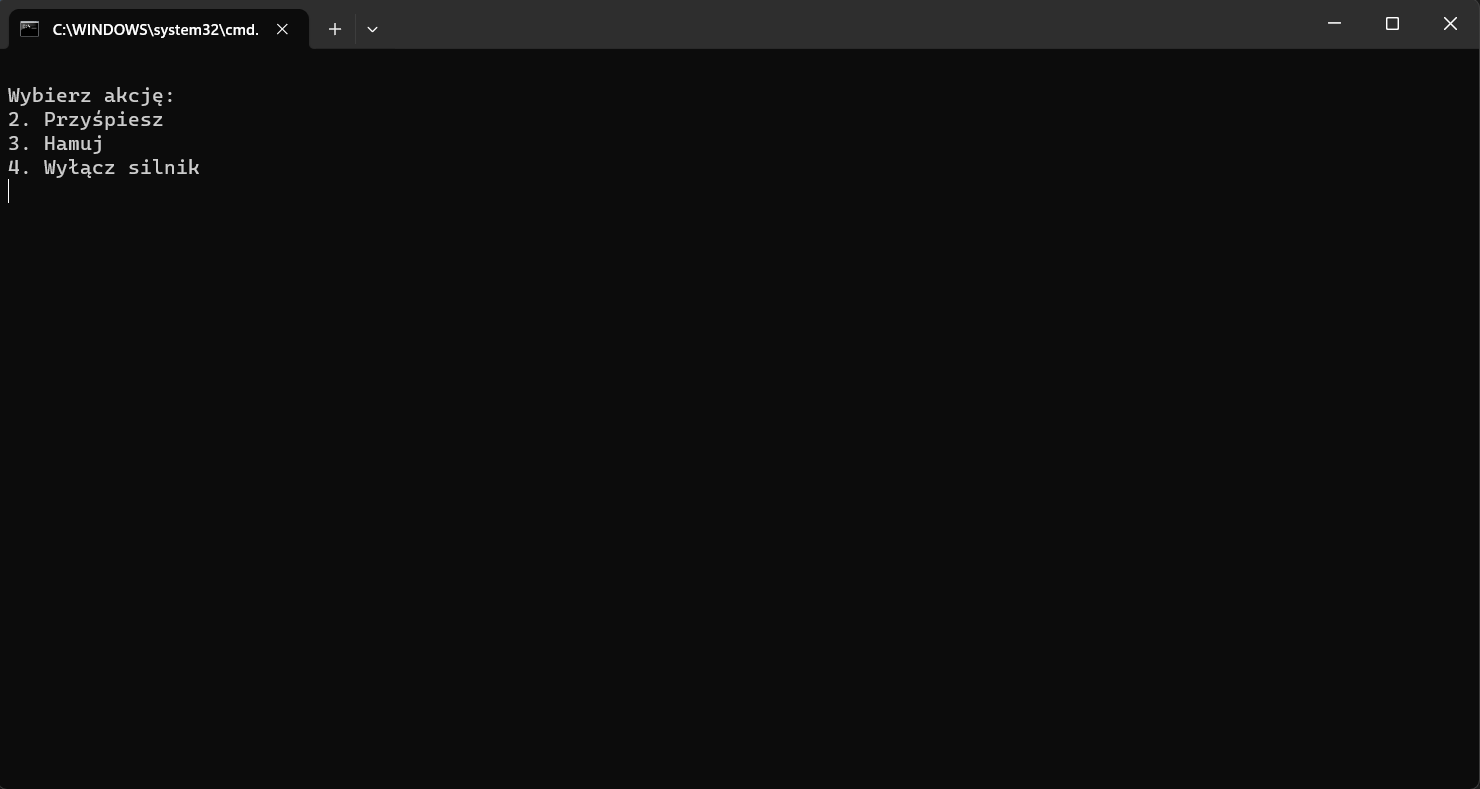
\includegraphics[width=17cm]{Wyłączenie silnika.png}
	\caption{\footnotesize Wyłączenie silnika}
	\label{fig:plotend}
\end{figure}
% ********** Koniec rozdziału **********
